\documentclass[10pt,a4paper] {article}
\usepackage{epsf}
\usepackage{latexsym}
\usepackage{hyperref}
\usepackage{graphicx}
\setlength{\textheight}{22.5cm} 
\setlength{\textwidth}{16cm}
\setlength{\oddsidemargin}{2.5mm} 
\setlength{\topmargin}{0.1cm}
\setlength{\evensidemargin}{-5mm}

%% Definitions
\newcommand {\hide}[1] {\typeout{ #1 }}
%Comment out to print all
%\newcommand {\hide}[1] {{\it #1 }}
%Comment out to hide some
\newcommand{\beq}{\begin{equation}}
\newcommand{\eeq}{\end{equation}}
\newcommand{\dif}[2]{\frac{{\rm d} #1}{{\rm d} #2}}
\newcommand{\ildif}[2]{{\rm d} #1/{{\rm d} #2 }}
\newcommand{\ilpdif}[2]{\partial #1/{\partial #2 }}
\newcommand{\pdif}[2]{\frac{\partial #1}{\partial #2}}
\newcommand{\pddif}[3]{\frac{\partial^2 #1}{\partial #2 \partial #3}}
\newcommand{\ilpddif}[3]{\partial^2 #1/{\partial #2 \partial #3}}
\newcommand{\bm}[1]{\mbox{\boldmath $#1$}}
\newcommand{\comb}[2]{\left (\begin{array}{c}{#1}\\{#2}\end{array}\right )}
\newcommand{\gfrac}[2]{\mbox{$ { \textstyle{ \frac{#1}{#2} }\displaystyle}$}}

% comment out next line unless double spacing needed
%\renewcommand{\baselinestretch}{2}


\begin {document}
\begin{center}
{\Large \bf PyDDE 0.2.2: \\a cross-platform numerical solver for systems of delay differential equations with switches.\\}
\vspace{0.3cm}
Benjamin J. Cairns,\\ Cancer Epidemiology Unit, University of Oxford, \\Richard Doll Building, Roosevelt Drive, Oxford OX3 7LF, \textsc{United Kingdom}.\\ {\tt %%@
ben.cairns@ceu.ox.ac.uk}
\end{center}

\tableofcontents

\section{Introduction}

PyDDE is derived from a MS Windows DDE solver named Solv95.  The introduction to the original Solv95 manual begins as follows:

\begin{quotation}
Solv95 is designed to allow numerical solution of systems of ordinary and delay differential equations, which may have state variable discontinuities (switches). To use it you need a C/C++ compiler/linker capable of producing 32 bit Windows executables with a graphical user interface.  Suitable compiler/linkers are supplied commercially by Borland or Microsoft (these come with quite useful debugging facilities), or you can use GNU C/C++ for Windows, which is available without charge (but has slightly less user friendly debugging tools).  To solve a set of equations you must edit a template C file to specify the model. This is then compiled and linked to the numerical and graphical routines which will solve the model and display the results.
\end{quotation}

PyDDE is built around numerical routines that originally appeared as Solv95, using instead the GPL-licensed \verb+ddesolve+ package for the the \verb+R+ statistical computing environment as a source, to which I have been a contributor.  (A version of PyDDE pre-dating \verb+ddesolve+ was adapted directly from the non-GPL Solv95 code, but I contributed code to \verb+ddesolve+ that returns states at user-specified times, and it makes sense to keep a single codebase.)  In any case, both PyDDE and \verb+ddesolve+ remove the Microsoft Windows-specific graphical user interface code and wrap the integration routines in nice, scriptable packages.  For PyDDE specifically, this means that on most systems the Solv95 DDE solver can be installed as a Python package.  No specific C compiler is required; Python takes care of the compilation process at first installation.  The routines are accessed entirely from within Python, so that rather than editing a template C file, users may specify---and subsequently edit---their models using Python scripts.

PyDDE's advantages are the same as those of Solv95 and \verb+ddesolve+.  It is designed to solve delay differential equations (but will happily solve ordinary differential equations also) with or without discontinuities in state (``switches'').  The environment in which PyDDE is built (that is, Python) is freely available, and both Python and PyDDE are open source.  Some of the disadvantages of Solv95 are fixed or mitigated in PyDDE (and, yes, also in \verb+ddesolve+).  It allows more rapid prototyping of models, makes the solution of the equations more readily available to further analysis or display using other Python packages and does a little more checking of errors.  The wrapping of the C code was done `by hand' (rather than using SWIG or similar tools) and so it may be inelegant.  Suggestions for improvement of any aspect of the wrapping code are most welcome.

Solv95 was written by Simon N. Wood.  I obtained a copy of the source in December 2005 under the following conditions:
\begin{quotation}The package is provided on condition that the following be accepted: (i) The package comes with %%@
no warrenty and remains the property of the author. (ii) The package and compiled models may be %%@
re-distributed, provided that no charge is made for doing so, original authorship is fully %%@
acknowledged and these conditions are accepted by the recipient.\end{quotation}
However, the authors of \verb+ddesolve+ (obtained October 2007) have been permitted by Simon Wood to release that package's source under the GPL, so PyDDE is also available under the GPL.  Please see the package contents for a copy of the license.  In addition to license-mandated acknowledgements, I would particularly like to acknowledge the authorship of Solv95 by Simon Wood; his work makes PyDDE possible, where mine merely makes it available.  I would also like to thank the authors of \verb+ddesolve+---Alex Couture-Beil, Jon T. Schnute, and Rowan Haigh---who have done a terrific job porting Solv95 to \verb+R+, and were very welcoming of my proposed additions.  Thanks also to Josh Lippai of Pomona College, who squashed a bug that caused a compilation error on some OS X systems.

Finally, please note that PyDDE is based on \verb+ddesolve+, and I had wanted to keep some parity between version numbers between the two projects.  Due to the need to for occasional revisions to fix bugs and so on this is not really possible.  The current version of PyDDE (0.2.2) has the same back-end as version 1.0.1 of \verb+ddesolve+.  There are remarkably few differences between the two; the only discrepancies boil down to replacing \verb+R+-specific code with Python-specific code.  All the real work is done purely in C.  ``Mileage may vary,'' as they say, but all other things being equal the two solvers should produce identical results.

\section{Installing PyDDE}

The package has been successfully installed and used on a variety of Apple Mac systems, including a PowerMac G5 and a MacBook Intel Core 2 Duo,  with OS 10.4.x, on Python 2.3, 2.4 and 2.5, \verb+gcc+ 4.0.x.  It has also been successfully installed on a Microsoft Windows XP SP2 system running Python 2.4.1 installed through Cygwin and \verb+gcc+ 3.x.

In order to use PyDDE you will need to have Python installed with the Numeric or NumPy packages.  Numeric or NumPy can be obtained from 
\begin{quotation}\url{http://numeric.scipy.org/}\end{quotation}
and
\begin{quotation}\url{http://numpy.scipy.org/}\end{quotation}
If you install or wish to use Numeric but not NumPy, see the note below.  If your system doesn't have a Python distribution included, you can almost certainly find one to suit your needs at
\begin{quotation}\url{http://www.python.org/}\end{quotation}
respectively.  Note that some combinations of Python and Numeric/NumPy tend to be faster than others.  For example, using Numeric 24.2, calculations for the included test.py take an average of 3.30 seconds with Python 2.3.5 (OS X version), but only 2.27 seconds on 2.4.3 (DarwinPorts) and 2.82 seconds on 2.5.0 (DarwinPorts).  Again on Python 2.5.0 (DarwinPorts), but with with NumPy 1.0.2 instead of Numeric, it takes 2.88 seconds.

You will also (normally) need access to the same compiler that was used to create your Python distribution.  If you installed Python from a binary (executable) and you find that PyDDE won't install because you don't have the right compiler, there are various ways to fix the situation.  PyDDE may be available as a binary for some distributions (particularly MS Windows); check the PyDDE web page for more information. Alternatively, you could try installing Python another way (e.g. using Fink on an Apple OS 10.x machine or Cygwin on a Microsoft Windows machine)!

I have received reports that current versions of NumPy do not automatically copy the required header files to Python's \verb+include+ directory.  To make these available, simply copy (or add a symbolic link to) the \verb+numpy/core/include/numpy+ directory from your Python distribution's \verb+site-packages+ directory into your Python distribution's \verb+include+ directory, e.g. \verb+/usr/local/include/python2.5/+.  For example, on a UNIX-style system, you could type:
\begin{verbatim}
  cd /usr/local/include/python2.5/
  ln -s /usr/local/lib/python2.5/site-packages/numpy/core/include/numpy numpy
\end{verbatim}
You should, of course, modify these commands to match your own system.  (Thanks to Josh Lippai for this information.)

\subsection{Numeric vs. NumPy}

Starting with version 0.2.1, PyDDE depends on NumPy.  However, PyDDE does not presently take advantage of any of the array addressing or C-API improvements in NumPy.  Thus, it is possible to get PyDDE working with the older Numeric, instead.  To achieve this, change the line
\begin{quotation}\verb+#include <numpy/arrayobject.h>+\end{quotation}
in the file \verb+wrapper.c+ to read
\begin{quotation}\verb+#include <Numeric/arrayobject.h>+\end{quotation}
to maintain backwards compatibility, or even
\begin{quotation}\verb+#include <numpy/oldnumeric.h>+\end{quotation}
if you are feeling contrarian.  More about NumPy and SciPy can be found at
\begin{quotation}\url{http://www.scipy.org/}\end{quotation}

\subsection{Detailed installation instructions}

PyDDE is installed like many other Python packages.  First, if you have not 
already done so download the latest source distribution from:
\begin{quotation}\url{http://seis.bris.ac.uk/~bzzbjc/python/PyDDE/}\end{quotation}
Unpack the source distribution to a suitable location, open a command or 
terminal window, change to the root directory of the source distribution (which 
will contain setup.py) and type:
\begin{quotation}\verb+$ python setup.py install+\end{quotation}
Of course, if you usually type something else to start Python running, replace
\verb+python+ in the above with that command.  That should be all that is necessary but read on if you have trouble.  

If you'd like to add any further compiler flags, such as -msse3 for further optimisation of code, you can do so by editing the \verb+extra_compile_args+ field in setup.py.  This is currently empty (i.e. ``'') but could be set to any string that makes sense for your compiler (e.g. ``\verb+-msse3+''; note that the addition of the -msse flag seems to have little or no effect on run times, but your mileage may vary).

If you have a version of Python earlier than 2.4, you will probably receive a warning:  
\begin{quotation}\verb+UserWarning: Unknown distribution option: `package_data'+\end{quotation}
This may be safely ignored, but if this happens you will need to make a copy of the PyDDE documentation (the PDF and/or TeX files in the \verb+./doc+ directory of the
distribution) if you want it for future reference.

Note that if you don't have Numeric or NumPy installed, you should get an error during installation as these are required at compilation time.  You may also get warnings (rather than errors) from the C compiler used by Python to
install the module; these may (usually!) be safely ignored.


\section{Defining models}

Solv95's manual has this to say about the kind of problems it is designed to solve:
\begin{quotation}
The program aims to solve problems of the general form:
\begin{eqnarray*} 
\dif{s_0}{t} & = & g_0 ({\bf s}(t),{\bf s}(t-\tau_0), {\bf s}(t-\tau_1), \ldots,t)\\
\dif{s_1}{t} & = & g_1 ({\bf s}(t),{\bf s}(t-\tau_0), {\bf s}(t-\tau_1), \ldots,t)\\
\dif{s_2}{t} & = & g_2 ({\bf s}(t),{\bf s}(t-\tau_0), {\bf s}(t-\tau_1), \ldots,t)\\
. & . & ~~~~~~~~~. \\
. & . & ~~~~~~~~~. 
\end{eqnarray*}
subject to initial conditions on the $s_i$'s, and with the possible addition of some discontinuities in the $s_i$'s.  The $s_i$'s are the {\it state variables } of the problem and ${\bf s}(t)$ is used to mean the vector of all state variables at time $ t$, so $ {\bf s}(t-\tau)$ is the vector of state variables time $\tau $ ago.  To define a model the user must specificy the functions $g_i$ which return the gradients of $s_i$ w.r.t. time given the state variables at time $t$ and at a series of lagged times.  The user must also specify the starting values for all state variables.
\end{quotation}
As with Solv95, models are defined in PyDDE by providing a variety of information and some functions to the solver.  The first step is in all cases to import the appropriate package(s) and then create an instance of the \verb+dde+ class.  You may find it useful to follow these instructions in Python in order to get some practice in using PyDDE.

\begin{verbatim}
  from PyDDE import pydde
\end{verbatim}

Note that PyDDE is distributed as a Python package, containing the two modules pydde and ddesolve.  Only pydde should be used directly by the user under normal circumstances, so this is what we import.  

\subsection{A DDE example}

As an example, we'll consider the delay differential equation example that comes with Solv95: Nicholson's~(1954) blowfly model from Gurney and Nisbet~(1981).  This model is a one-dimensional delay differential equation:
$$
\dif{A}{t}= \left\{ \begin{array} {lc}
- \delta A(t), & t < \tau, \\
P A(t-\tau) e^{-A(t-\tau)/A_0} - \delta A(t), & t \ge \tau, \end{array} \right.
$$
where $ A $ is the population of adult flies in a laboratory population, $ \tau$ is the %%@
development time from egg to adulthood, $P$ is maximum adult fecundity rate multiplied by the %%@
survival rate from egg to adult, and $A_0$ is a parameter determining how quickly fecundity %%@
declines with adult population.  (The above description was taken directly from the Solv95 manual.)

Setting up this model and solving it in PyDDE is remarkably easy.  First, we make sure everything is imported from the scipy or Numeric packages to give access to array creation and exponential functions, and then create a new instance of the \verb+pydde.dde+ class:
\begin{verbatim}
  from scipy import *
  dde_eg = pydde.dde()
\end{verbatim}
Then next step is to define the gradient function,
\begin{verbatim}
  def ddegrad(s, c, t):
      alag = 0.0
      if (t>c[0]):
          alag = pydde.pastvalue(0,t-c[0],0)
      return array( [ c[2]*alag*exp(-alag/c[3])-c[1]*s[0] ] )
\end{verbatim}
Observe that this is a function of the state \verb+s+ (an array of floats), a float array of constants \verb+c+ and the scalar float time \verb+t+.  These are always the types of the arguments of the gradient function, so keep that in mind when constructing models: always access the first dimension of the state as \verb+s[0]+ even when the model is only one-dimensional.  

In this model, the constant \verb+c[0]+ gives the delay at which to calculate the state, but observe that we only calculate this if the time is greater than this delay.  It is important to know that no history of the process is provided \emph{by the algorithm} earlier than time~$0$.  However, a sort of initial history can be provided by replacing the line \verb+alag = 0+ with \verb+alag = func(t-c[0])+ where \verb+func+ is some known function.  It is important to remember that asking for past values or gradients from earlier than time~$0$ using \verb+pydde.pastvalue+ or \verb+pydde.pastgradient+ may produce errors, and the behaviour of the solver in such cases is officially undefined.  It is the user's responsibility to ensure that such requests are never made.

You will have noticed that the function \verb+grd+ uses \verb+pydde.pastvalue+; this function does exactly what it says, giving (an interpolated estimate of) the state of the process at a time prior to the current time.  It takes three arguments.  First, a non-negative integer describes which of the history variables to report.  Second, a scalar float gives the time at which to obtain the value of the selected history variable.  Third, a non-negative integer describes which lag (that is, delay) this is; from comments in the template files of Solv95:
\begin{quotation}
[L]ag pointers are used by \verb+pastvalue+ to store the history buffer location corresponding to a lag in order to save exectution time.  For example if your code requires lagged varaible 0 at lags T and 2T for each gradient calculation then it is efficient to obtain these values using: \verb+pastvalue(0,t-T,0)+ and \verb+pastvalue(0,t-2*T,1)+ rather than \verb+pastvalue(0,t-T,0)+ and \verb+pastvalue(0,t-2*T,0)+.  The latter works, it's just slower because more time is spent searching for lagged values.
\end{quotation}
In this case we do not use \verb+pastgradient+, but this provides the gradient of the process at a time prior to the current time and takes exactly the same arguments.

When there are delays in the model, it is important to also define a function to store the history variables.  By default, the solver will use the state and gradient values as the history variables; this is just what we want in this case, but in general we must ensure that when using this default, the number of history variables is the same as the number of state variables.  If we wanted to go ahead and define the history storage function anyway, we could use
\begin{verbatim}
  def ddesthist(g, s, c, t):
      return (s, g)
\end{verbatim}
which must return a tuple containing float arrays of the appropriate sizes.  Note that the arguments of this function are the same as for the gradient function, plus the float array \verb+g+ defining the gradient of the state variables at time \verb+t+.

The next step is to initialise the model as an attribute of \verb+dde_eg+.  We will achieve this by defining the constants and initial conditions and a state-scaling array for use in error control when values are very close to~$0$.

\begin{verbatim}
  ddecons = array([12.0,0.25,10.0,300.0,100.0])
  ddeist = array([ddecons[4]])
  ddestsc = array([0])
\end{verbatim}

At last, we can initialise the problem---that is, define the model---by calling the \verb+initproblem+ method of \verb+dde_eg+:
\begin{verbatim}
  dde_eg.initproblem(no_vars=1, no_cons=5, nhv=1, nlag=1, nsw=0, no_otimes=301,
                     t0=0.0, t1=300.0,
                     initstate=ddeist, c=ddecons, 
                     otimes=numpy.arange(0.0, 300.0, 1.0),
                     grad=ddegrad, storehistory=ddesthist)
\end{verbatim}
The arguments of this method are, respectively, the number of state variables \verb+no_vars+, the number of constants \verb+no_cons+, the number of history variables \verb+nhv+, the number of lags or delays \verb+nlag+ (for the third argument of \verb+pastvalue+), the number of switches or discontinuities \verb+nsw+, the number of output times \verb+no_otimes+, the initial time \verb+t0+, the final time \verb+t1+, the initial conditions \verb+initstate+, the constants \verb+c+, the times at which to output the state \verb+otimes+, the gradient function \verb+grad+ and the history storage function \verb+storehistory+.  (Note that the `switch' functions \verb+switchfunctions+ and the map functions \verb+maps+ to be applied when switches are triggered are not specified here as there are no switches.)  Some error checking is performed and then these data are recorded in \verb+dde_eg.PROB+.  Note that the solver will assume that, for example, \verb+no_cons+ agrees with the length of the constants array \verb+c+.  Behaviour of the solver when these assumptions are broken is, again, officially undefined, but some error checking is performed to ensure that the output of the supplied functions agrees with the number of state variables, constants and so on.  

The final step before solving the model is to initialise the solver.  This is done in a similar fashion to the initialisation of the model, using the \verb+initsolver+ method:
\begin{verbatim}
  dde_eg.initsolver(tol=0.000005, hbsize=1000,
                    dt=1.0, statescale=ddestsc)
\end{verbatim}
The arguments of this method are the tolerance for use in error calculations \verb+tol+, the size of the history buffer \verb+hbsize+, the initial time-step of the solver \verb+dt+ and the state-scaling values \verb+statescale+.  These data are recorded in \verb+dde_eg.SOLVER+.

At last, we can solve the model, using the method \verb+solve+:
\begin{verbatim}
  dde_eg.solve()
\end{verbatim}
This method usually takes no arguments (but see below), as everything is provided in the \verb+dde_eg.PROB+ and \verb+dde_eg.SOLVER+ tuples.  It produces roughly \verb+(t1-t0)/dout+ observations of the process, placing the values of the state variables in the array \verb+dde_eg.data+, with one column for each of the state variables, and placing the times of these values in the array \verb+dde_eg.t+.  These observations are now available for further analysis, plotting, storage etc.  

If the solver appears to have been successful, the \verb+solve()+ method will also set a flag to indicate that the solver has completed.  Repeated calls to \verb+solve()+ will then have no effect, other than printing a message stating that the problem has already been solved and reminding the user of the location of the \verb+data+ and \verb+t+ attributes.  To force the solver to re-run, use \verb+solve(again=1)+.

\subsection{Example, abbreviated}

``What a drawn out waste of time!'' you say.  ``I just want to run a single command, just a few arguments, and have it solve the thing then and there.'' 

I agree.  Starting with version 0.2.1, PyDDE has an alternative, simplified interface that is much like that of \verb+ddesolve+ or \verb+odesolve+ from \verb+R+.  Instead of the above you could simply use the command
\begin{verbatim}
  dde_eg.dde(y=ddeist, times=numpy.arange(0.0, 300.0, 1.0), 
             func=ddegrad, parms=ddecons, 
             tol=0.000005, dt=1.0, hbsize=1000, nlag=1, ssc=ddestsc)
\end{verbatim}
The internals of the \verb+dde.dde()+ method take care of the initialisation steps, but some options are not available (for example the number of history variables is the same as the number of elements of \verb+y+).  For good or bad, the names of the arguments to this function differ from those of \verb+initproblem+ and \verb+initsolver+ so that they match the names of arguments to the \verb+dde()+ function in the \verb+R+ package \verb+ddesolve+.

For further details on the various functions and their usage, please see the original Solv95 manual (which should have been provided with this manual in the file \verb+solv95manual.pdf+).  The module \verb+PyDDE.ddesolve+ incorporates all the functions and data necessary for use of the Solv95 program, and the following sections detail their use in PyDDE.  (Note that \verb+PyDDE.ddesolve+ is automatically loaded by \verb+PyDDE.pydde+.)

\subsection{Function arguments}

The following subsections describe the various arguments to the \verb+initproblem+, \verb+initsolver+ and \verb+dde+ functions.  Again, the names of arguments differ in \verb+dde+ so as to match those of the equivalent function from the \verb+R+ package \verb+ddesolve+.

\subsubsection{\tt{grad} \textrm{(or} {\tt func}\textrm{ in} {\tt dde()}\textrm{)}}\label{S:grad}

The gradient function specifies the differential equations which define the system to be solved.  There is little to be said for the gradient function that is specific to PyDDE, except that the functions \verb+pastvalue+ and \verb+pastgradient+ referred to in the Solv95 manual's description of this function are available as \verb+pydde.pastvalue+ and \verb+pydde.pastgradient+.  The function should return a float array of length \verb+no_vars+.

\subsubsection{\tt{storehistory}} 

The default value for \verb+storehistory+ is a function that simply returns the tuple \verb+(s,g)+ as the history, but in principle any function of \verb+g+, \verb+s+, \verb+c+ and \verb+t+, returning values and associated gradients to be stored, is appropriate.  It is recommended that the default function, defined as
\begin{verbatim}
  storehistory=(lambda g,s,c,t: (array(s),array(g)))
\end{verbatim}
be used in most circumstances, and any computations required on these variables when calculating gradients with \verb+pydde.pastvalue+ or \verb+pydde.pastgradient+ be done in the gradient function.  In some cases, to save on memory requirements it may be advisable to record only those state variables and gradients that are actually needed for calculations in the gradient function.  For example, if there were $6$ state variables, and only the first, second and fifth were required, we would set \verb+nhv=3+ and a suitable history storage function might be
\begin{verbatim}
  def storefunc(g, s, c, t):
      return (array([s[0],s[1],s[4]]), array([g[0],g[1],g[4]]))
\end{verbatim}

In general, the history storage function should return a tuple of two float arrays, each with length \verb+nhv+.  It is important that the second of these arrays actually contain the gradients of the first, as calculations of the history at arbitrary times uses both the history values and their gradients.

\subsubsection{\tt{initstate} \textrm{(or} {\tt y}\textrm{ in} {\tt dde()}\textrm{)}}

In Solv95 the initial state of the process is provided by a user-defined function, \verb+initstate+.  PyDDE contains such a function, hidden in the PyDDE.ddesolve module, but the initial state of the process is provided by the user as a float array of length \verb+no_vars+.

\subsubsection{\tt{statescale} \textrm{(or} {\tt ssc}\textrm{ in} {\tt dde()}\textrm{)}}

From the Solv95 manual:
\begin{quotation}
Solv95 controls integration error by specifying that it should be less than some specified %%@
proportion of each state variable.  This can cause difficulties when some state variables are in %%@
the vicinity of zero.  For example, if a state variable is at zero, but about to leave that state, %%@
then the integrator may attempt to estimate that variable with zero error - which requires a zero %%@
timestep!  The solution adopted is to get the user to specify a small number to be added to the %%@
magnitude of each state variable when estimating proportianal integration error.
\end{quotation}
In PyDDE, the user supplies a float array of \verb+no_vars+ values to be added in such error calculations.  If this array is the wrong length, it will either be truncated or padded with $0$'s until it is the correct length, but note that no notification or warning will be issued to this effect.

\subsubsection{\tt{switchfunctions} \textrm{(or} {\tt switchfunc}\textrm{ in} {\tt dde()}\textrm{)}}

Switch functions are defined such that a `switch' or discontinuity is triggered whenever one of the switch varibles passes through zero from positive to negative.  Switch functions should do this smoothly and not more than once per time step, so it may be important to set the solver parameters such as \verb+maxdtx+ so that this does not occur.  The Python switch function defined by the user should return a float array with the same length as the problem parameter \verb+nsw+.  When a switch is triggered, integration is suspended and the number of the switch function (between $0$ and \verb+nsw+) is passed to the function \verb+map+.

A simple example of a switch function is one that is triggered once, when the time \verb+t+ is equal to the value of the first constant \verb+c[0]+:
\begin{verbatim}
  def swfun(s, c, t):
      return array([c[0]-t])
\end{verbatim}

Note that there's no reason why a switch function can't contain one or more random components, provided that these random times can be evaluated prior to defining the switch function.  State-dependent random switch times may be technically feasible, but are likely to mess with the accuracy of the simulation.  Thus, PyDDE can also be used to simulate a sub-class of piecewise-determinisitic Markov processes (PDMPs) with random deviations with state-independent timings.

\subsubsection{\tt{maps} \textrm{(or} {\tt mapfunc}\textrm{ in} {\tt dde()}\textrm{)}}

The map function must return both the array of state variables (of length \verb+no_vars+) and the array of constants (of length \verb+no_cons+) to be valid.  A simple example is one which does nothing, regardless of the switch number:
\begin{verbatim}
  def mapfunc(s, c, t, swno):
      return (s,c)
\end{verbatim}
Note that \emph{this is the only function in which the constants can be changed} and so they must be returned, but may be returned unchanged.  A slightly more complicated example, from the Solv95 manual, is
\begin{verbatim}
  def mapfunc(s, c, t, swno):
      rets = s
      if (swno==0):
          rets[0] *= 2
          rets[1] *= 2 
      elif (swno==1):
          rets[0] *= c[0]/t
      return (rets,c)
\end{verbatim}

Just as with switch functions, map functions may have a random component, but unlike in switch functions, these random terms may be evaluated during the simulation, and may be state-dependent in any way that can be expressed using Python.

\subsection{Utility functions}

The following functions provide access to delayed state variables and gradients.  They are primarily intended for use inside user-specified gradient functions (see \S\ref{S:grad}).

\subsubsection{\tt pydde.pastvalue}

The function \verb+pastvalue+ in the PyDDE.pydde module is used in exactly the same way as \verb+pastvalue+ from Solv95; the first argument is the index of the history variable to return, the second is the time at which the history variable should be calculated, and the third is the index of the lag `marker'.  This final variable can be safely set to $0$ in all cases, but is better set to a unique value for each unique lag (that is, delay) in the model.

Once again, it is important that the requested times are not from earlier than \verb+t0+ (or, for that matter, from later than the current time!).  Initial histories---values for times less than \verb+t0+---can be coded within the gradient function \verb+grad+.

Note that \verb+pastvalue+ should usually recognise badly formatted input (it attempts to cast arguments suitably before calling on the underlying routine), but if this fails it will return a (float) value of 0.

\subsubsection{\tt pydde.pastgradient}

The function \verb+pastgradient+ provides the gradient of a history variable in exactly the same way as \verb+pastvalue+ provides the states.  However, since it is defined by the function \verb+storehistory+, the values obtained using \verb+pastgradient+ could be anything at all.  If these values are indeed the gradients, the Solv95 manual notes:
\begin{quotation}
... its use is somewhat dubious, since the order of approximation of the interpolated gradients is lower than the order of approximation of the integrator which may lead to infelicities in the numerical solution of models using this function.
\end{quotation}

The function \verb+pastgradient+ has the same behaviour as \verb+pastvalue+ in case of errors in argument types.

\section{Test examples}

Examples are provided in the file \verb+test/test.py+ in the PyDDE distribution directory.  These examples are the same models provided as examples with Solv95: an ODE model, a DDE model and an `SDDE' model (a DDE model with switches).

The figures that follow were produced using the pyx package for producing plots in Python; the code to produce these graphics forms part of \verb+test.py+.

\begin{figure}[bp]
\begin{center}
\scalebox{0.96}{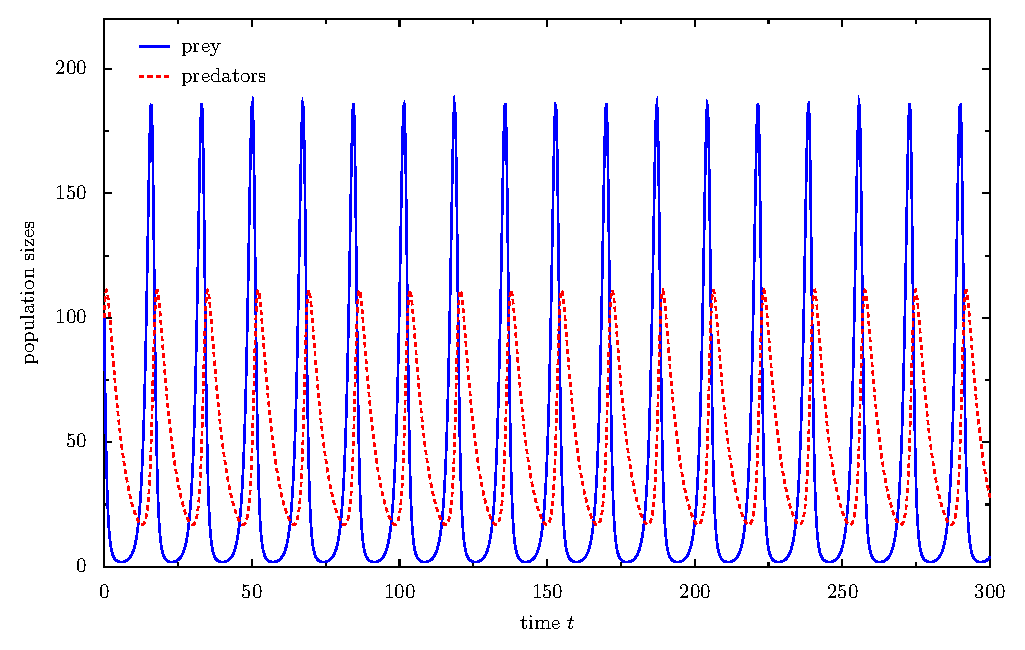
\includegraphics{./ode_eg.eps}}
\caption{A Lotka-Volterra predator-prey system (ODE).}\label{fig:ode}
\end{center}
\end{figure}

\begin{figure}[bp]
\begin{center}
\scalebox{0.96}{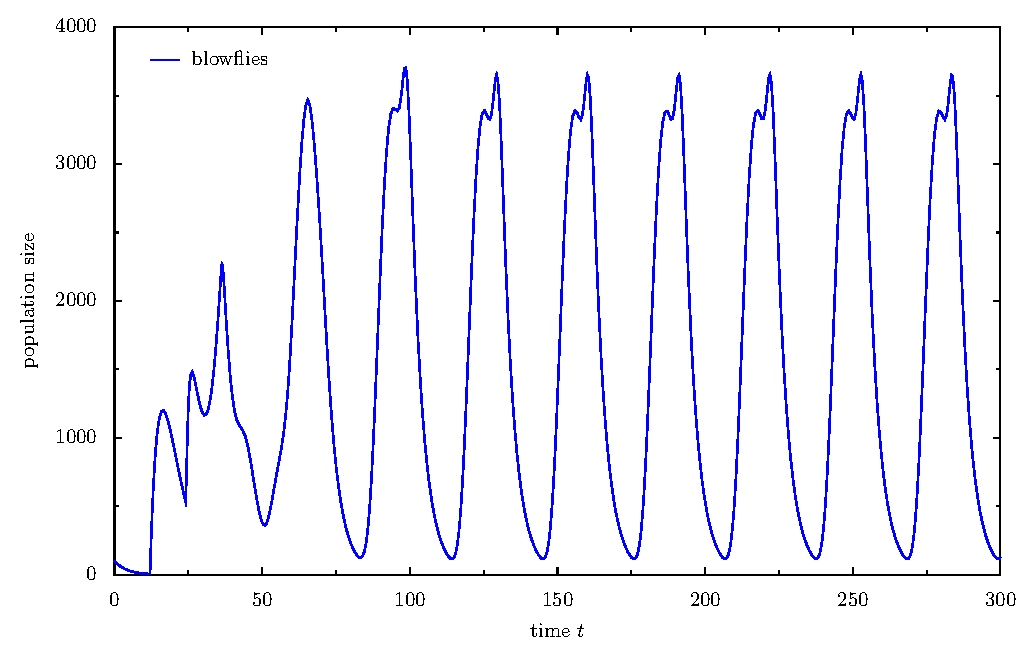
\includegraphics{./dde_eg.eps}}
\caption{Gurney and Nisbet's (1981) model of Nicholson's (1954) blowflies (DDE).}\label{fig:dde}
\end{center}
\end{figure}

\begin{figure}[bp]
\begin{center}
\scalebox{0.96}{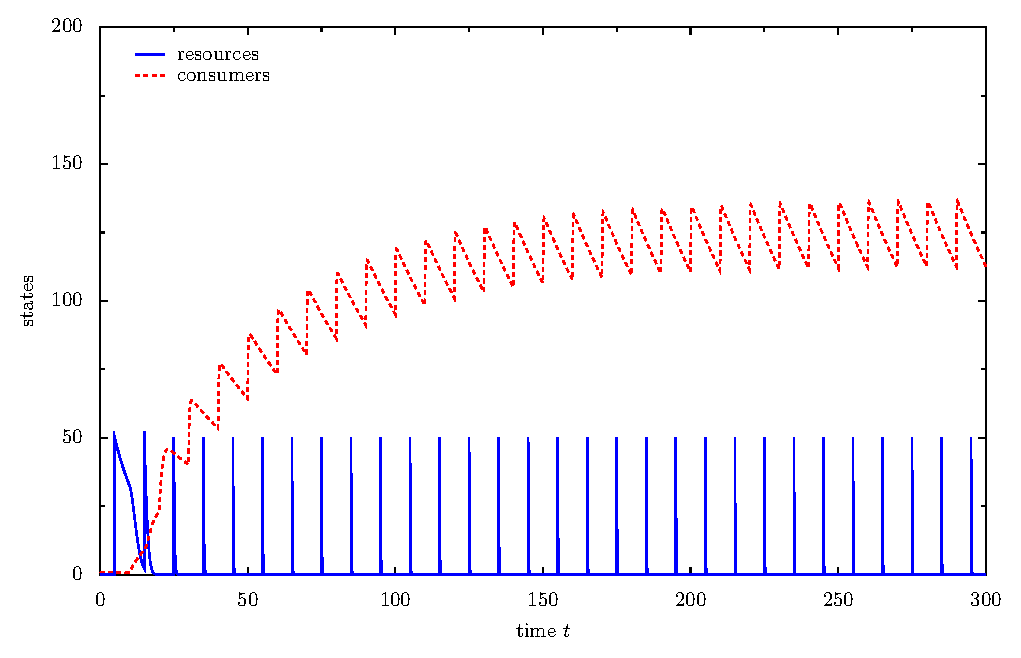
\includegraphics{./sdde_eg.eps}}
\caption{A model for a population of consumers feeding on a resource that is replenished at regular intervals (SDDE).}\label{fig:sdde}
\end{center}
\end{figure}

\section{The algorithm}

For details of the algorithm and references, please see the Solv95 manual.
  
\end{document}
